\begin{frame}[allowframebreaks]{}
    \LARGE Normalizing Flow Models: \\[1.5ex] \textbf{Jacobian (2D Case)}
\end{frame}

\begin{frame}[allowframebreaks]{Jacobian (2D Case)}
\begin{itemize}
    \item The Jacobian is a matrix of partial derivatives:
    \[
    J_{ij} = \frac{\partial f_i}{\partial z_j}
    \]
    \item It describes how each component of $f(z)$ changes with $z$.
    \item The Jacobian is needed to compute how volumes change after transformation.
\end{itemize}

\framebreak

\begin{figure}
    \centering
    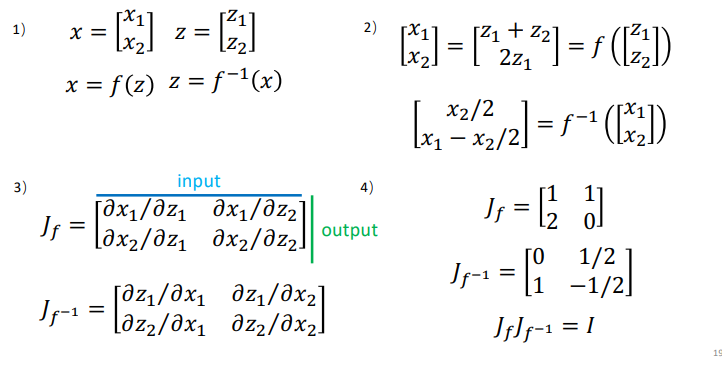
\includegraphics[height=0.8\textheight, width=\textwidth, keepaspectratio]{images/norm-flow/jacobian.png}
    \caption*{Example of a 2D Jacobian matrix. See Appendix~\ref{sec:appendix-jacobian-2d} for more information.}
\end{figure}
    
\end{frame}